\begin{remark*}[Exposition]
The preceding metrics become metric spaces once their domains are paired with
the verified distance functions.  This section records the resulting spaces as
objects in their own right.
\end{remark*}

\begin{definitionbox}{Definition --- Vacuous Metric on Empty Types}
\begin{definition}[Vacuous Metric on Empty Types]
\label{def:vacuous-metric-empty-types}
Let \(X\) be an empty type.  The \emph{vacuous metric} on \(X\) is the unique
function
\[
  d_{\varnothing}:X\times X\to\mathbb{R}_{\geq 0}.
\]
\end{definition}
\end{definitionbox}

\begin{remark*}[Standard quantified statement]
\[
X=\varnothing
\Longrightarrow
d_{\varnothing}:X\times X\to\mathbb{R}_{\geq 0}.
\]
All metric axioms hold vacuously because there are no points of \(X\).
\end{remark*}

\begin{remark*}[Interpretation]
An empty type has no pairs of points and therefore no nontrivial distance
values.  The metric axioms impose no additional conditions.
\end{remark*}

\LeanFormalizes{def:vacuous-metric-empty-types}{lra-lean}{LRA.VolumeIV.MetricSpaces.Metrics}{VacuousMetric}{statement}

\DefinitionalRoot

\begin{definitionbox}{Definition --- Empty Subtype Metric}
\begin{definition}[Empty Subtype Metric]\label{def:empty-subtype-metric}
Let \((X,d)\) be a metric space, and let
\[
  \varnothing_X:=\{x\in X : \text{false}\}.
\]
The \emph{empty subtype metric} is the restriction of \(d\) to
\(\varnothing_X\).
\end{definition}
\end{definitionbox}

\begin{remark*}[Standard quantified statement]
\[
d_{\varnothing_X}:
\varnothing_X\times\varnothing_X\to\mathbb{R}_{\geq 0},
\qquad
d_{\varnothing_X}(x,y)=d(x,y).
\]
\end{remark*}

\begin{remark*}[Interpretation]
The empty subtype metric is the inherited metric on an empty subset.  Since
the subset has no points, the inherited metric axioms are vacuous.
\end{remark*}

\LeanFormalizes{def:empty-subtype-metric}{lra-lean}{LRA.VolumeIV.MetricSpaces.Metrics}{EmptyMetric}{statement}

\DefinitionalRoot

\begin{propositionbox}{Proposition}
\begin{proposition}[The Empty Set is a Metric Space]
\label{prop:empty-set-metric-space}
The empty set equipped with its vacuous metric is a metric space.

\smallskip
\noindent
\hyperref[prf:empty-set-metric-space]{\textit{Go to proof.}}
\end{proposition}
\end{propositionbox}

\begin{remark*}[Standard quantified statement]
\[
  \varnothing=\{x:x\neq x\},
  \qquad
  \mathsf{MetricSpace}(\varnothing,d_{\varnothing}).
\]
\end{remark*}

\begin{remark*}[Predicate reading]
\[
\varnothing=\{x:x\neq x\},
\qquad
\mathsf{MetricSpace}(\varnothing,d_{\varnothing})
\]
means that the empty set carries the metric-space structure whose metric
axioms hold vacuously.
\end{remark*}

\begin{remark*}[Interpretation]
The empty metric space is the degenerate metric space with no points and no
distances to check.
\end{remark*}

\LeanFormalizes{prop:empty-set-metric-space}{lra-lean}{LRA.VolumeIV.MetricSpaces}{EmptySetIsAMetricSpace}{checked}

\begin{dependencies}
\begin{itemize}
  \item \hyperref[def:metric-space]{Definition: Metric Space}
  \item \hyperref[def:vacuous-metric-empty-types]{Definition: Vacuous Metric on Empty Types}
  \item \hyperref[def:empty-subtype-metric]{Definition: Empty Subtype Metric}
\end{itemize}
\end{dependencies}

\begin{definitionbox}{Definition --- Singleton Subtype Metric}
\begin{definition}[Singleton Subtype Metric]\label{def:singleton-subtype-metric}
Let \((X,d)\) be a metric space and let \(a\in X\).  On the singleton
\(\{a\}\), the \emph{singleton subtype metric} is the restriction of \(d\) to
\(\{a\}\).  Equivalently, every pair of points in \(\{a\}\) has distance
\(0\).
\end{definition}
\end{definitionbox}

\begin{remark*}[Standard quantified statement]
\[
d_{\{a\}}:\{a\}\times\{a\}\to\mathbb{R}_{\geq 0},
\qquad
d_{\{a\}}(x,y)=d(x,y)=0.
\]
\end{remark*}

\begin{remark*}[Interpretation]
A singleton has only one point, so the only distance value forced by the
metric axioms is the distance from that point to itself.
\end{remark*}

\LeanFormalizes{def:singleton-subtype-metric}{lra-lean}{LRA.VolumeIV.MetricSpaces.Metrics}{SingletonMetric}{statement}

\DefinitionalRoot

\begin{propositionbox}{Proposition}
\begin{proposition}[A Singleton Set is a Metric Space]
\label{prop:singleton-set-metric-space}
Every singleton set equipped with its singleton subtype metric is a metric
space.

\smallskip
\noindent
\hyperref[prf:singleton-set-metric-space]{\textit{Go to proof.}}
\end{proposition}
\end{propositionbox}

\begin{remark*}[Standard quantified statement]
\[
a\in X
\Longrightarrow
\mathsf{MetricSpace}(\{a\},d_{\{a\}}).
\]
\end{remark*}

\begin{remark*}[Predicate reading]
\[
\mathsf{MetricSpace}(\{a\},d_{\{a\}})
\]
means that the inherited singleton distance satisfies the metric axioms on
\(\{a\}\).
\end{remark*}

\begin{remark*}[Interpretation]
The singleton metric space is the one-point metric space.  All metric
comparisons collapse to the identity distance \(d(a,a)=0\).
\end{remark*}

\LeanFormalizes{prop:singleton-set-metric-space}{lra-lean}{LRA.VolumeIV.MetricSpaces}{SingletonSetIsAMetricSpace}{checked}

\begin{dependencies}
\begin{itemize}
  \item \hyperref[def:metric-space]{Definition: Metric Space}
  \item \hyperref[def:singleton-subtype-metric]{Definition: Singleton Subtype Metric}
\end{itemize}
\end{dependencies}

\begin{definitionbox}{Definition --- Discrete Metric Space}
\begin{definition}[Discrete Metric Space]\label{def:discrete-metric-space}
Let \(X\) be a nonempty set.  The \emph{discrete metric space on \(X\)} is the
metric space
\[
  (X,d_{\mathrm{disc}}),
\]
where \(d_{\mathrm{disc}}\) is the discrete metric on \(X\).
\end{definition}
\end{definitionbox}

\begin{remark*}[Standard quantified statement]
\[
X\neq\varnothing
\Longrightarrow
\operatorname{MetricSpace}(X,d_{\mathrm{disc}}).
\]
\end{remark*}

\begin{remark*}[Interpretation]
A discrete metric space is a space where distinct points are all separated by
the same positive distance.  Its geometry records equality and inequality, but
no finer notion of nearness.
\end{remark*}

\begin{dependencies}
\begin{itemize}
  \item \hyperref[def:metric-space]{Definition: Metric Space}
  \item \hyperref[def:discrete-metric]{Definition: Discrete Metric}
  \item \hyperref[prop:discrete-metric-space]{Proposition: The Discrete Distance is a Metric}
\end{itemize}
\end{dependencies}

\begin{definitionbox}{Definition --- Euclidean Metric Space}
\begin{definition}[Euclidean Metric Space]\label{def:euclidean-metric-space}
For \(n\in\mathbb{N}\), the \emph{standard Euclidean metric space} is
\[
  (\mathbb{R}^n,d_2),
\]
where \(d_2\) is the Euclidean metric on \(\mathbb{R}^n\).
\end{definition}
\end{definitionbox}

\begin{remark*}[Standard quantified statement]
\[
n\in\mathbb{N}
\Longrightarrow
\operatorname{MetricSpace}(\mathbb{R}^n,d_2).
\]
\end{remark*}

\begin{remark*}[Interpretation]
The Euclidean metric space is the standard finite-dimensional distance model:
points are coordinate vectors, and distance is ordinary straight-line length.
\end{remark*}

\begin{dependencies}
\begin{itemize}
  \item \hyperref[def:metric-space]{Definition: Metric Space}
  \item \hyperref[def:euclidean-space]{Definition: Euclidean Space}
  \item \hyperref[def:euclidean-distance-rn]{Definition: Euclidean Distance on \(\mathbb{R}^n\)}
  \item \hyperref[cor:euclidean-metric]{Corollary: Euclidean Metric}
\end{itemize}
\end{dependencies}

\begin{definitionbox}{Definition --- Taxicab Metric Space}
\begin{definition}[Taxicab Metric Space]\label{def:taxicab-metric-space}
For \(n\in\mathbb{N}\), the \emph{taxicab metric space} is
\[
  (\mathbb{R}^n,d_1),
\]
where \(d_1\) is the taxicab metric on \(\mathbb{R}^n\).
\end{definition}
\end{definitionbox}

\begin{remark*}[Standard quantified statement]
\[
n\in\mathbb{N}
\Longrightarrow
\operatorname{MetricSpace}(\mathbb{R}^n,d_1).
\]
\end{remark*}

\begin{remark*}[Interpretation]
The taxicab metric space has the same underlying set as Euclidean space, but
distance is measured by summing coordinatewise displacements.
\end{remark*}

\begin{dependencies}
\begin{itemize}
  \item \hyperref[def:metric-space]{Definition: Metric Space}
  \item \hyperref[def:taxicab-metric-rn]{Definition: Taxicab Metric}
  \item \hyperref[prop:taxicab-metric-rn]{Proposition: Taxicab Metric}
\end{itemize}
\end{dependencies}

\begin{definitionbox}{Definition --- \(p\)-Metric Space}
\begin{definition}[\(p\)-Metric Space]\label{def:lp-metric-space}
Let \(1\leq p<\infty\) and let \(n\in\mathbb{N}\).  The \emph{\(p\)-metric
space} is
\[
  (\mathbb{R}^n,d_p),
\]
where \(d_p\) is the \(p\)-metric on \(\mathbb{R}^n\).
\end{definition}
\end{definitionbox}

\begin{remark*}[Standard quantified statement]
\[
1\leq p<\infty,\; n\in\mathbb{N}
\Longrightarrow
\operatorname{MetricSpace}(\mathbb{R}^n,d_p).
\]
\end{remark*}

\begin{remark*}[Interpretation]
The \(p\)-metric spaces form a family of finite-dimensional metric spaces on
the same coordinate set, with different rules for turning coordinate
displacements into distance.
\end{remark*}

\begin{figure}[htbp]
\centering
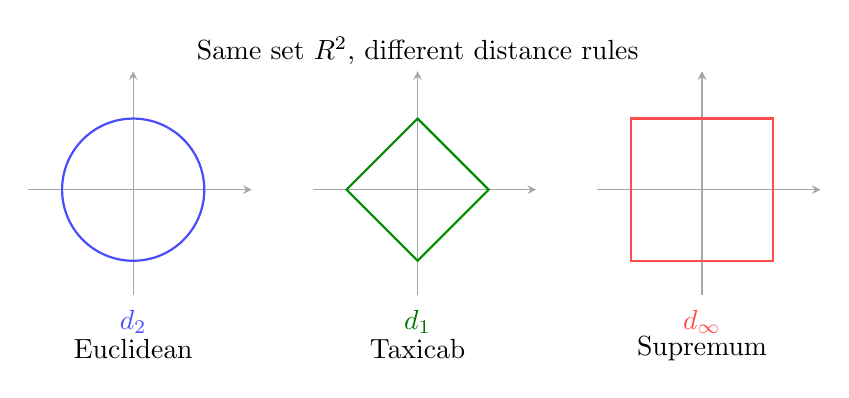
\begin{tikzpicture}[scale=0.86,>=stealth]
  \draw[->,gray!70] (-1.55,0) -- (1.75,0);
  \draw[->,gray!70] (0,-1.55) -- (0,1.75);
  \draw[blue!70,thick] (0,0) circle (1.05);
  \node[blue!70] at (0,-1.95) {\(d_2\)};
  \node at (0,-2.35) {Euclidean};

  \begin{scope}[xshift=4.2cm]
    \draw[->,gray!70] (-1.55,0) -- (1.75,0);
    \draw[->,gray!70] (0,-1.55) -- (0,1.75);
    \draw[green!55!black,thick]
      (0,1.05) -- (1.05,0) -- (0,-1.05) -- (-1.05,0) -- cycle;
    \node[green!45!black] at (0,-1.95) {\(d_1\)};
    \node at (0,-2.35) {Taxicab};
  \end{scope}

  \begin{scope}[xshift=8.4cm]
    \draw[->,gray!70] (-1.55,0) -- (1.75,0);
    \draw[->,gray!70] (0,-1.55) -- (0,1.75);
    \draw[red!70,thick] (-1.05,-1.05) rectangle (1.05,1.05);
    \node[red!70] at (0,-1.95) {\(d_\infty\)};
    \node at (0,-2.35) {Supremum};
  \end{scope}

  \node[align=center] at (4.2,2.05)
    {Same set \(\mathbb{R}^2\), different distance rules};
\end{tikzpicture}

\caption{Different metrics on the same underlying set can produce different
metric shapes.  The unit ball in \(\mathbb{R}^2\) changes when distance is
measured by \(d_2\), \(d_1\), or \(d_\infty\).}
\label{fig:metric-unit-balls-r2}
\end{figure}

\begin{dependencies}
\begin{itemize}
  \item \hyperref[def:metric-space]{Definition: Metric Space}
  \item \hyperref[def:lp-metric-rn]{Definition: \(p\)-Metric on \(\mathbb{R}^n\)}
  \item \hyperref[thm:lp-metric-rn]{Theorem: \(d_p\) is a Metric}
\end{itemize}
\end{dependencies}

\begin{definitionbox}{Definition --- Complex Metric Space}
\begin{definition}[Complex Metric Space]\label{def:complex-metric-space}
The \emph{complex metric space} is
\[
  (\mathbb{C},d_{\mathbb{C}}),
\]
where \(d_{\mathbb{C}}\) is the usual Euclidean distance on the complex plane.
\end{definition}
\end{definitionbox}

\begin{remark*}[Standard quantified statement]
\[
\operatorname{MetricSpace}(\mathbb{C},d_{\mathbb{C}}).
\]
\end{remark*}

\begin{remark*}[Interpretation]
The complex metric space treats complex numbers as points in the Euclidean
plane, while retaining the notation and algebra of \(\mathbb{C}\).
\end{remark*}

\begin{dependencies}
\begin{itemize}
  \item \hyperref[def:metric-space]{Definition: Metric Space}
  \item \hyperref[def:complex-metric]{Definition: Complex Metric}
  \item \hyperref[prop:complex-plane-metric-space]{Proposition: The Complex Plane is a Metric Space}
\end{itemize}
\end{dependencies}

\begin{definitionbox}{Definition --- Bounded Sequence Metric Space}
\begin{definition}[Bounded Sequence Metric Space]
\label{def:bounded-sequence-metric-space}
The \emph{bounded sequence metric space} is
\[
  (\ell^\infty(\mathbb{R}),d_\infty),
\]
where \(\ell^\infty(\mathbb{R})\) is the set of bounded real sequences and
\(d_\infty\) is the supremum metric.
\end{definition}
\end{definitionbox}

\begin{remark*}[Standard quantified statement]
\[
\operatorname{MetricSpace}(\ell^\infty(\mathbb{R}),d_\infty).
\]
\end{remark*}

\begin{remark*}[Interpretation]
The bounded sequence metric space is an infinite-dimensional example.  Its
distance measures the largest coordinatewise discrepancy between two bounded
real sequences.
\end{remark*}

\begin{dependencies}
\begin{itemize}
  \item \hyperref[def:metric-space]{Definition: Metric Space}
  \item \hyperref[def:bounded-real-sequence-space]{Definition: Supremum Metric on Bounded Real Sequences}
  \item \hyperref[prop:bounded-real-sequence-space-sup-metric]{Proposition: Supremum Metric on Bounded Sequences}
\end{itemize}
\end{dependencies}
